\chapter{Implementation of Nearest Neighbor classification algorithm}
\section{Introduction}
In statistics, the k-nearest neighbors algorithm (k-NN) is a non-parametric classification method first developed by Evelyn Fix and Joseph Hodges in 1951, and later expanded by Thomas Cover. It is used for classification and regression. In both cases, the input consists of the k closest training examples in the feature space.
\begin{itemize}
    \item In k-NN classification, the output is a class membership. An object is classified by a majority vote of its neighbors, with the object being assigned to the class most common among its k nearest neighbors.
    \item In k-NN regression, the output is the property value for the object. This value is the average of the values of its k nearest neighbors.
\end{itemize}
\section{Preparing the dataset}
\subsection{Foreword}
We will be using the following libraries in this lab:
\begin{itemize}
    \item \textit{pandas} for loading and preprocessing the dataset.
    \item \textit{scikit-learn} for splitting the dataset into training and test sets and for implementing the k-NN algorithm as well as for calculating the accuracy of the model.
    \item \textit{math} for calculating the square root of a number.
\end{itemize}
\subsection{Selecting dataset}
In this lab, we will use the \textit{Breast Cancer\footnote{https://data.world/health/breast-cancer-wisconsin}} dataset. This dataset contains 569 samples of malignant and benign tumor cells. The first two columns in the dataset store the unique ID numbers of the samples and the corresponding diagnosis (M=malignant, B=benign), respectively. Columns 3-32 contain 30 real-valued features that have been computed from digitized images of the cell nuclei, which can be used to build a model to predict whether a tumor is benign or malignant.\\
From now on, we will use \textit{dataset} to refer to this dataset.

\subsection{Loading the dataset}
We will be using the \textit{pandas} library to load the dataset. The following code snippet shows how we can load the dataset using \textit{pandas}:
\begin{lstlisting}[language=Python]
    import pandas as pd
    df = pd.read_csv(
        'breast-cancer-wisconsin-data_data.csv', 
        usecols=lambda c: not c.startswith('Unnamed'))
\end{lstlisting}
\begin{figure}[h]
    \centering
    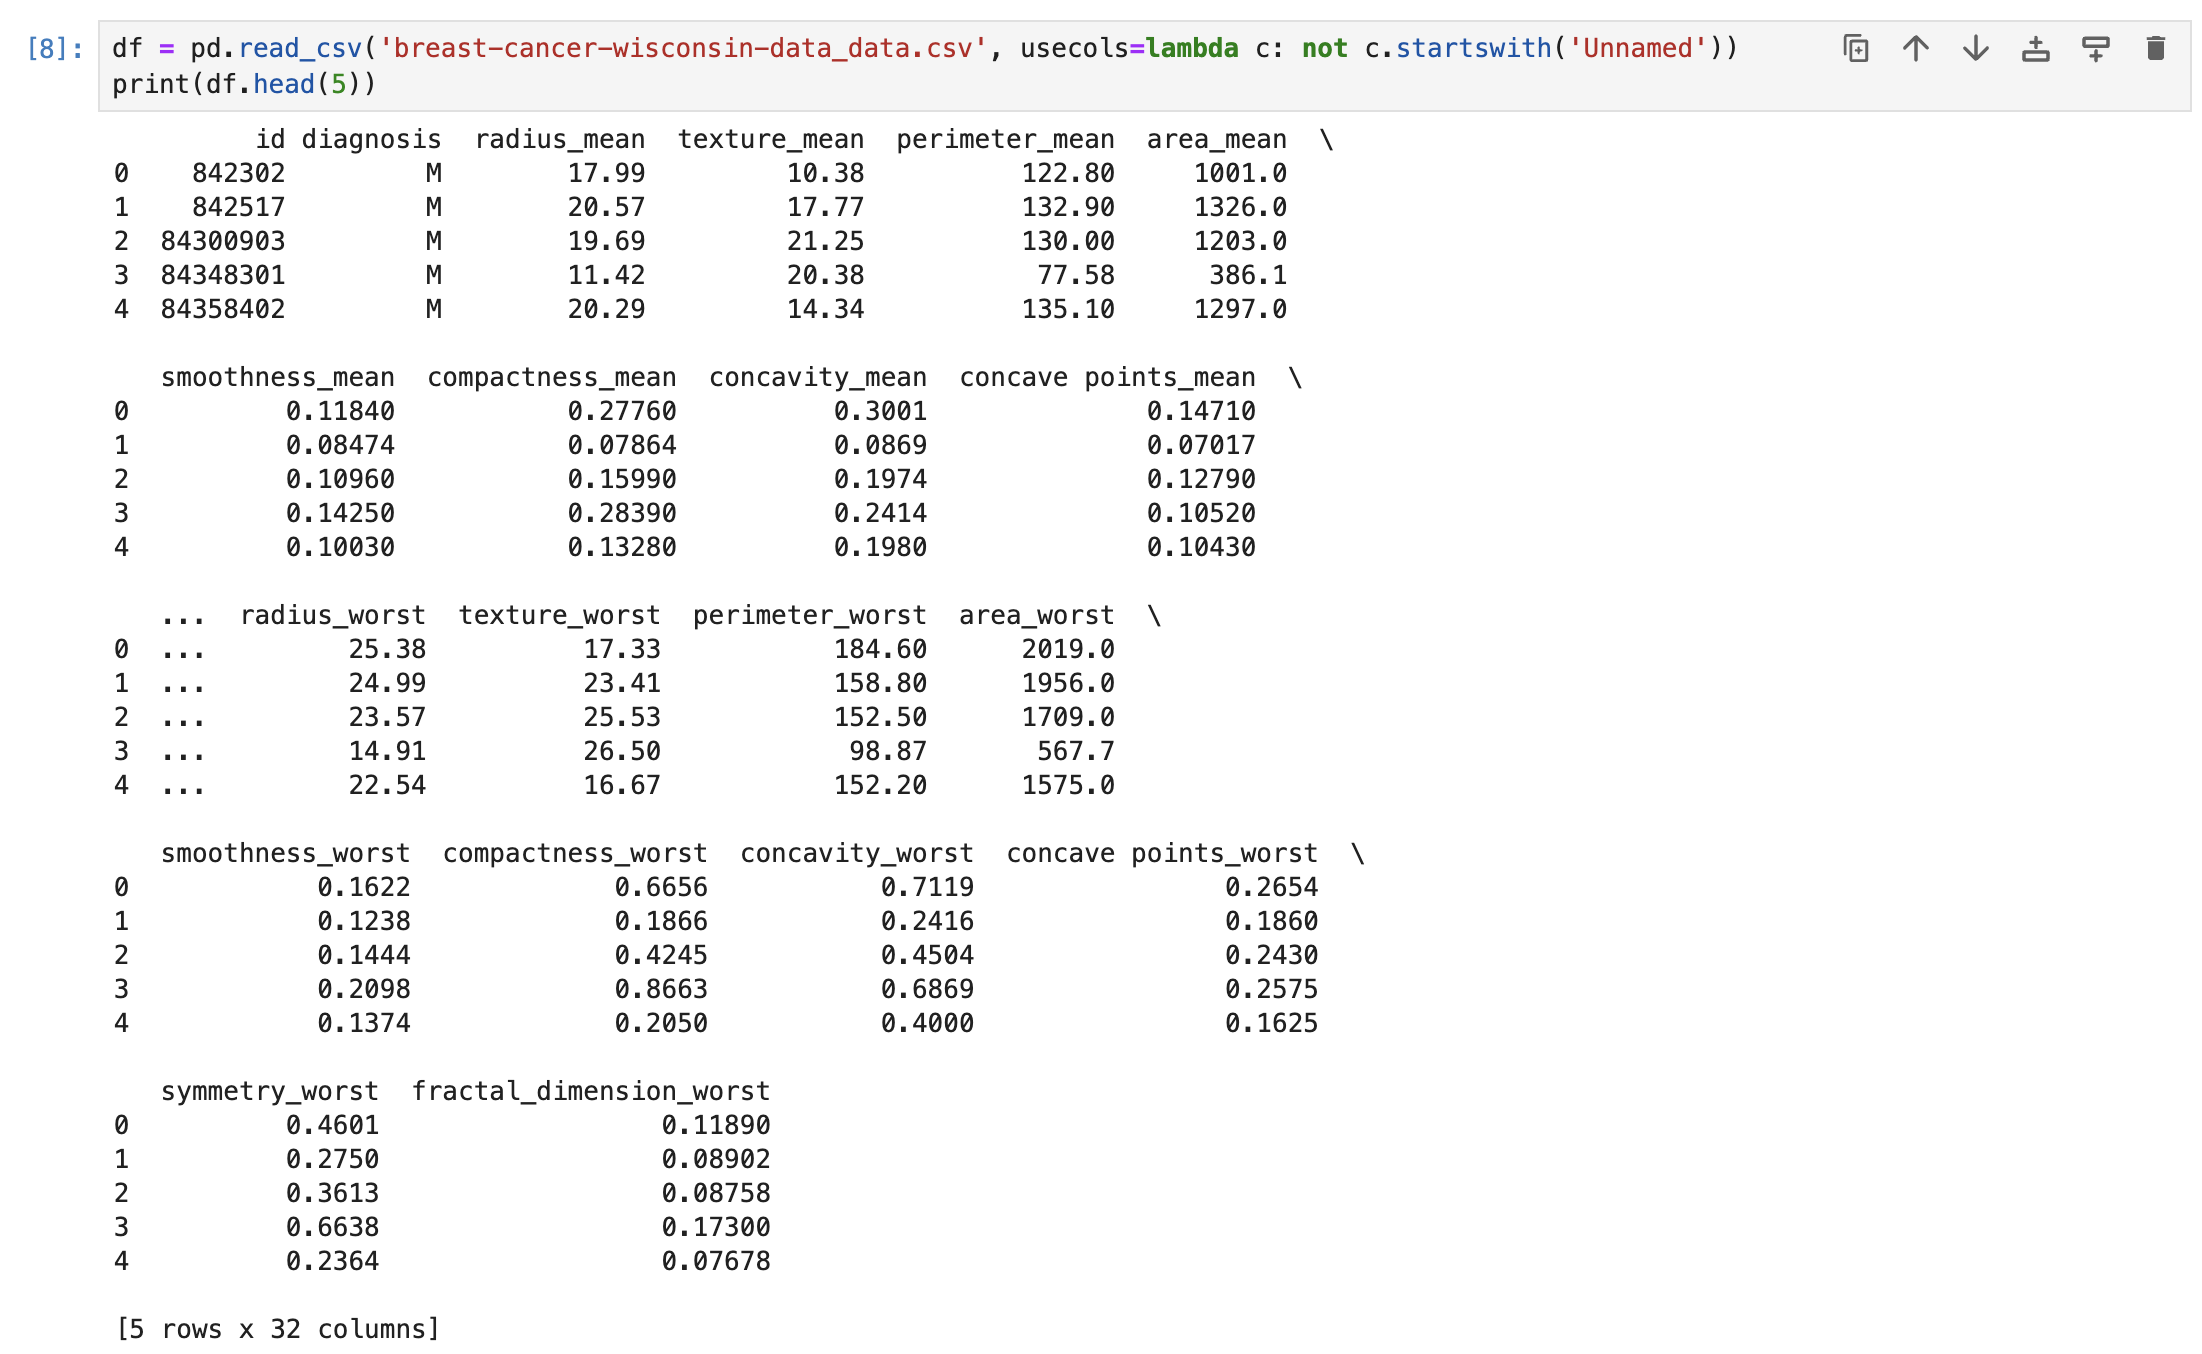
\includegraphics[width=15cm]{ch/figures/sneak-peek-into-dataset.png}
    \caption{A sneak peek into the dataset}
    \label{fig:sneak-peek-into-dataset}
\end{figure}
\subsection{Characteristics of the dataset}
There are some key characteristics of the dataset that we need to know before we start working with it.
To mention a few of them:
\begin{itemize}
    \item The dataset contains 569 samples.
    \item Each sample has 30 features.
    \item The dataset contains 212 malignant and 357 benign samples.
    \item The dataset contains no missing values.
\end{itemize}
This narrows down our task to the following, viz., our dataset has the following characteristics:
\begin{itemize}
    \item Size: 569 (i.e., 569 samples)
    \item Dimensionality: 30 (i.e., 30 features)
    \item Classes: 2 (i.e., 2 classes, malignant and benign)
    \item Ten real valued features are computed for each cell nucleus:
    \begin{itemize}
        \item Radius (mean of distances from center to points on the perimeter)
        \item Texture (standard deviation of gray-scale values)
        \item Perimeter
        \item Area
        \item Smoothness (local variation in radius lengths)
        \item Compactness (perimeter\textsuperscript{2} / area - 1.0)
        \item Concavity (severity of concave portions of the contour)
        \item Concave points (number of concave portions of the contour)
        \item Symmetry
        \item Fractal dimension ("coastline approximation" - 1)
    \end{itemize}
    \item Missing values: None
    \item Class distribution: 357 benign, 212 malignant
\end{itemize}
\subsection{Preprocessing the dataset}
To ease the process of working with the dataset, we will specifically preprocess the \textit{disagnosis} column of the dataset. We will replace the values \textit{M} and \textit{B} with 1 and 0 respectively. This will help us to work with the dataset more easily.
\begin{lstlisting}[language=Python]
    df['diagnosis'] = df['diagnosis']
                        .replace('M', 1)
    df['diagnosis'] = df['diagnosis']
                        .replace('B', 0)
\end{lstlisting}
\subsection{Selecting the features and the output}
We will be using the first 30 columns of the dataset as the features and the last column as the output. We will use the following code snippet to select the features and the output:
\begin{lstlisting}[language=Python]
    x = df.iloc[:, 2:32]
    y = df.iloc[:, 1]
\end{lstlisting}
\subsection{Splitting the dataset into training and test sets}
We will be using the \textit{scikit-learn} library to split the dataset into training and test sets. We will use the following code snippet to split the dataset into training and test sets:
\begin{lstlisting}[language=Python]
    X_train, 
    X_test, 
    y_train, 
    y_test = train_test_split(x, y, 
    test_size=0.2)
\end{lstlisting}
Here we have split the dataset into 80\% training set and 20\% test set.
\begin{figure}[h]
    \centering
    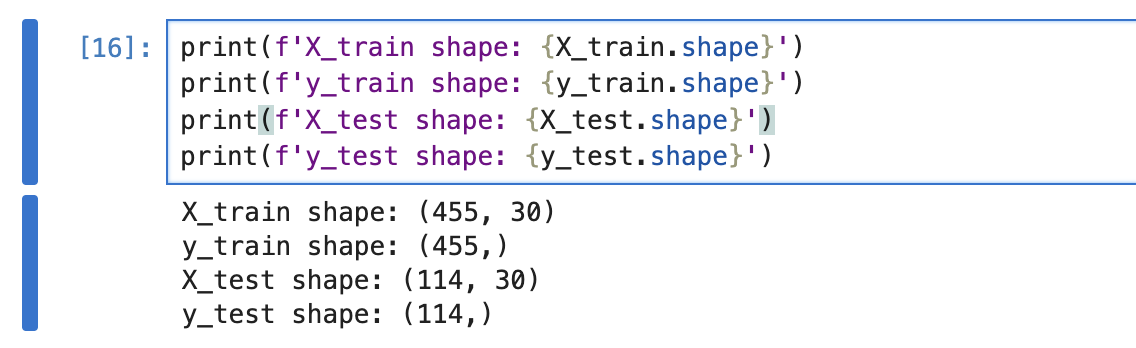
\includegraphics[width=10cm]{ch/figures/split-shape.png}
    \caption{Shape of the training and test sets}
    \label{fig:split-shape}
\end{figure}
\section{Implementing the k-NN algorithm}
\subsection{Selecting the value of k}
Value of k is a hyperparameter of the k-NN algorithm. Generally the value of k is selected as an odd number adjacent to the square root of the number of samples in the training set. In our case, the number of samples in the training set is 455. So, we will select the value of k as 21.
\begin{figure}[h]
    \centering
    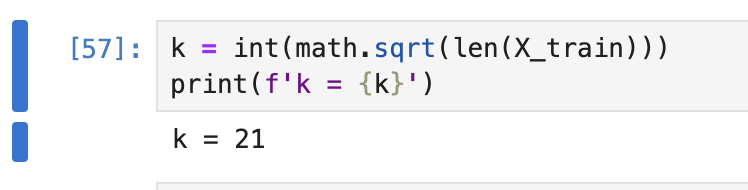
\includegraphics[width=10cm]{ch/figures/k-select.png}
    \caption{Selecting the value of k}
    \label{fig:ksel}
\end{figure}
\subsection{Calculating the distance between two samples}
There are several ways to calculate the distance between two samples. We will be using the Euclidean distance to calculate the distance between two samples.For Euclidean distance, we have to pass the following parameters to \textit{KNeighborsClassifier} class:
parameter \textit{metric} = \textit{euclidean}
\begin{lstlisting}[language=Python]
    classifier = KNeighborsClassifier(
        n_neighbors=21, 
        metric='euclidean')
\end{lstlisting}

\subsection{Training the model}
Now we can train the model using the following code snippet:
\begin{figure}[h]
    \centering
    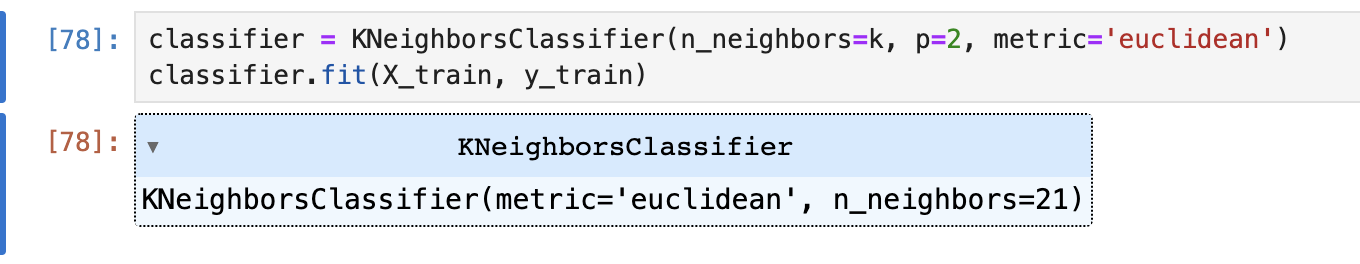
\includegraphics[width=10cm]{ch/figures/fit.png}
    \caption{Fitting the model}
    \label{fig:fit}
\end{figure}

\subsection{Predicting the output}
Now we can predict the output using the following code snippet:
\begin{lstlisting}
    y_pred = classifier.predict(X_test)
\end{lstlisting}

\section{Calculating the accuracy of the model}
There are several ways to calculate the accuracy of the model. 
We will be using the \textit{confusion matrix}, \textit{accuracy score} and \textit{f1 score} to calculate the accuracy of the model.
\subsection{Confusion matrix}
The confusion matrix is a technique used for summarizing the performance of a classification algorithm i.e. it has binary outputs. It is a table with 4 different combinations of predicted and actual values.
\begin{figure}[h]
    \centering
    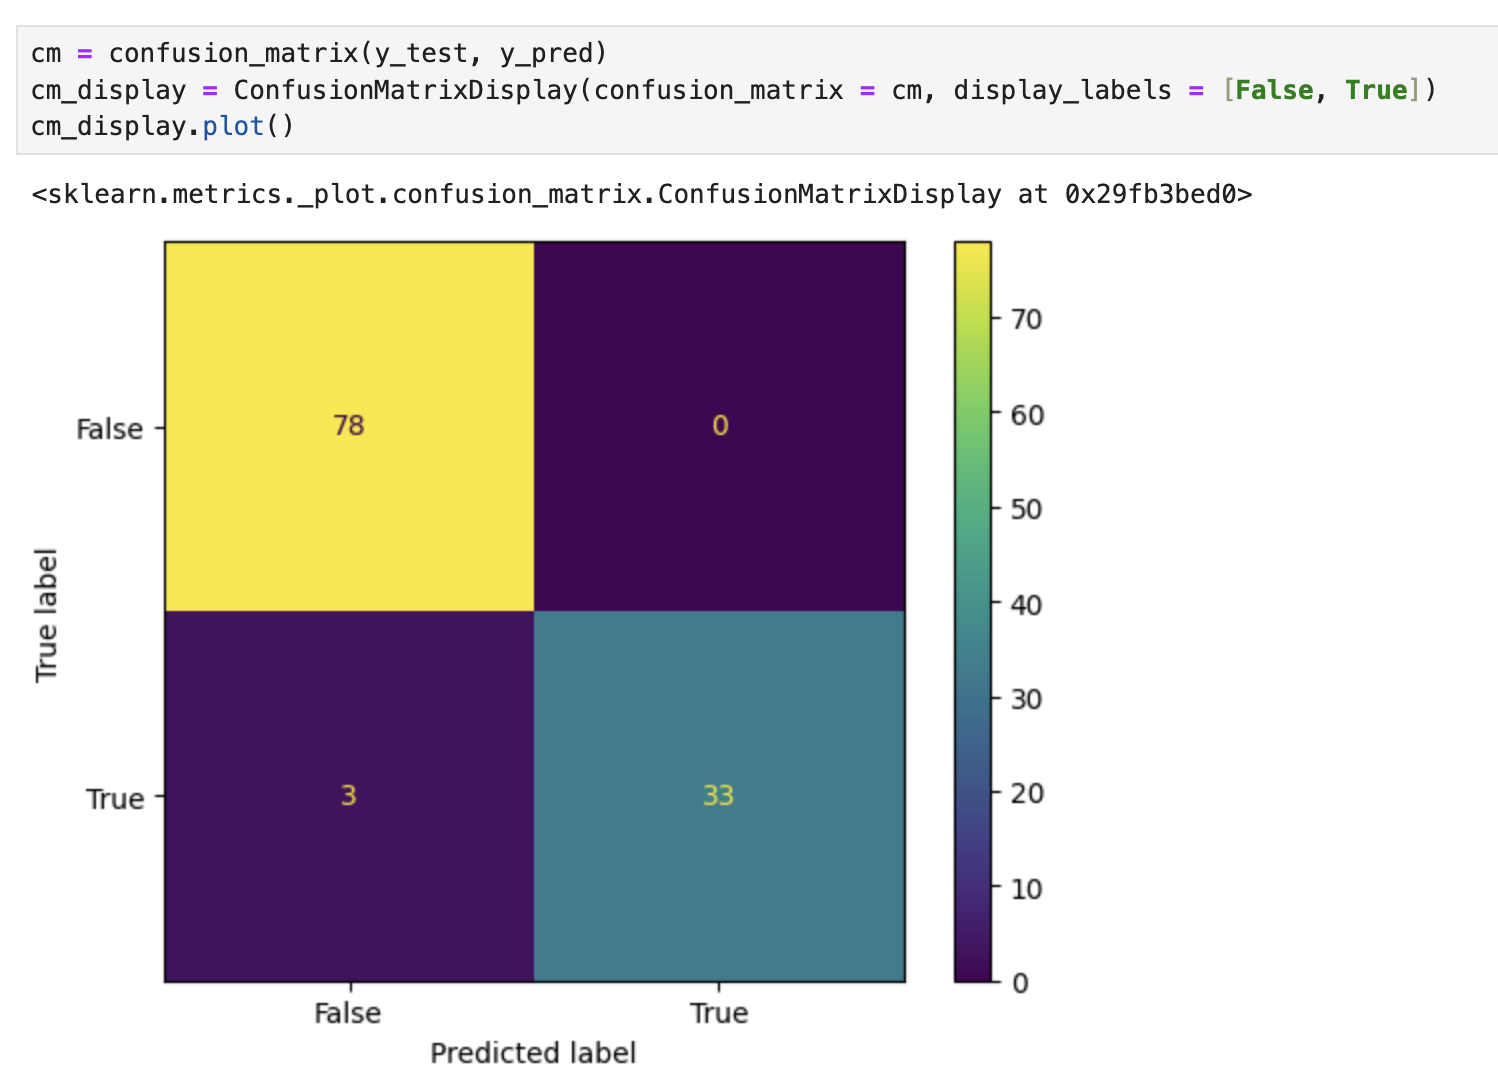
\includegraphics[width=12cm]{ch/figures/cm.png}
    \caption{Confusion matrix}
    \label{fig:cm}
\end{figure}
\newpage
\subsection{Accuracy score and f1 score}
\begin{figure}[h]
    \centering
    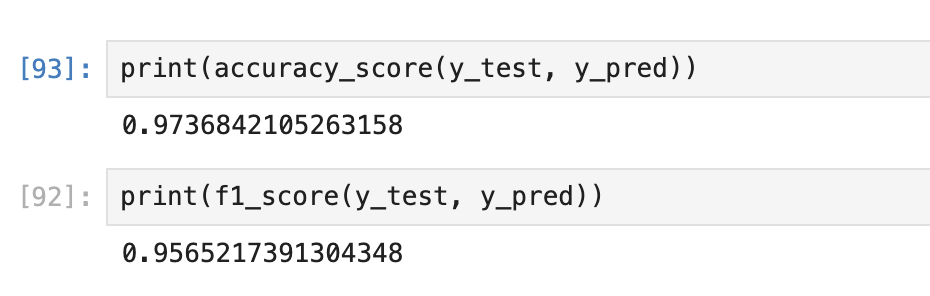
\includegraphics[width=12cm]{ch/figures/score.png}
    \caption{Score}
    \label{fig:score}
\end{figure}

\subsection{Relation between the value of \textit{k} and the accuracy of the model}
\begin{figure}[h]
    \centering
    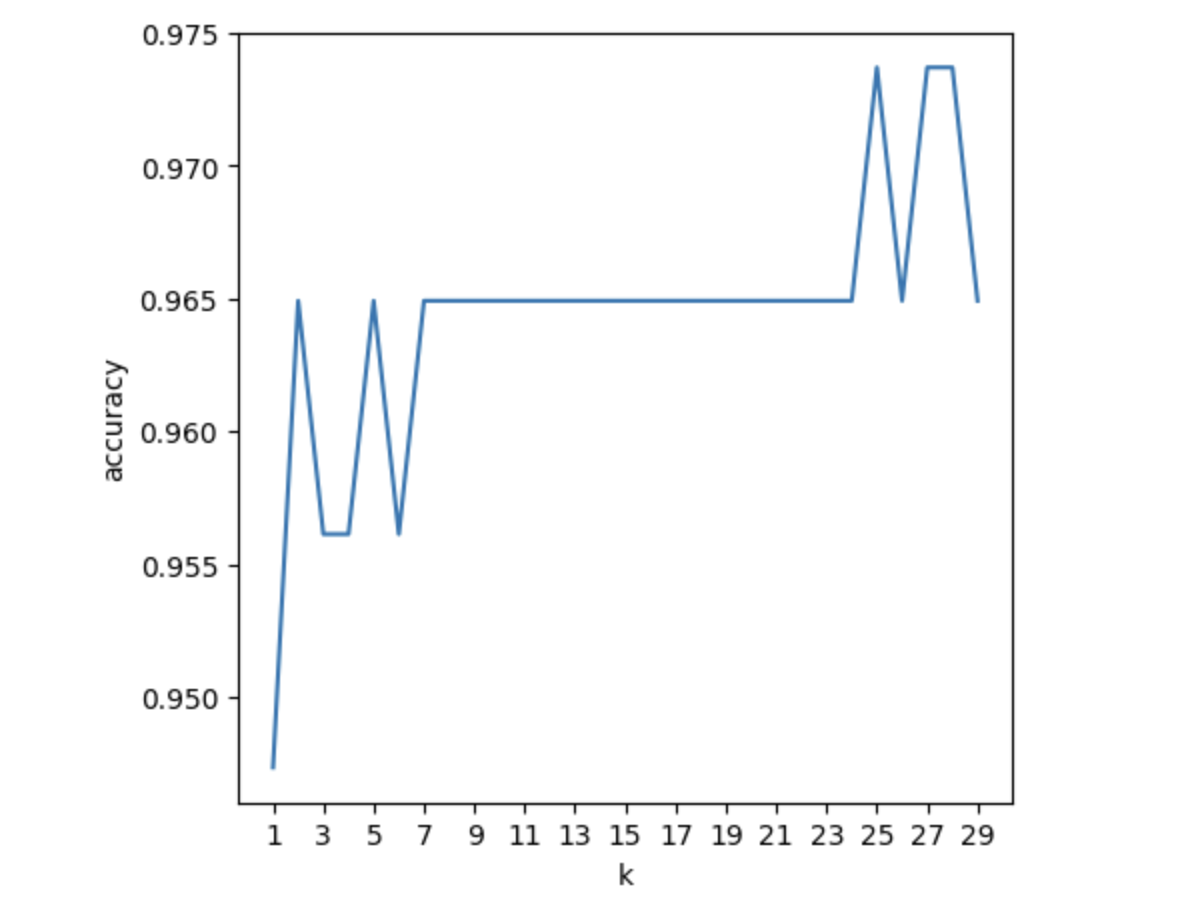
\includegraphics[width=12cm]{ch/figures/k-vs-score.png}
    \caption{Relation between the value of k and the accuracy of the model}
    \label{fig:k-acc}
\end{figure}
\newpage
\section{Drawbacks of the k-NN algorithm}
Some salient drawbacks of the k-NN algorithm are:
\begin{itemize}
    \item The k-NN algorithm is very sensitive to outliers.
    \item The k-NN algorithm is computationally expensive.
    \item The k-NN algorithm is not suitable for high dimensional data.
    \item The k-NN algorithm is not suitable for imbalanced data.
    \item The k-NN algorithm is not suitable for missing data.
    \item The k-NN algorithm is not suitable for large \\datasets.
    \item The k-NN algorithm is not suitable for noisy data.
\end{itemize}

\section{Conclusion}
In this lab, we have implemented the k-NN algorithm using the \textit{scikit-learn} library. We have also calculated the accuracy of the model using the \textit{confusion matrix}, \textit{accuracy score} and \textit{f1 score}. We have also discussed the drawbacks of the k-NN algorithm.